L'odierna rete elettrica è stata progettata come un sistema centralizzato, in cui l'energia elettrica fluisce attraverso linee unidirezionali di trasmissione e distribuzione dai generatori fino ai clienti finali. La logica applicativa è concentrata in zona centrale e solo parzialmente nelle \emph{substations}, mentre le componenti restanti sono totalmente passive. Le Smart Grid forniscono una più elevata ed ampia intelligenza distribuita incorporata nei dispositivi locali, comunicazione e scambio bidirezionale di informazioni ed elettricità.

\section{Smart Grid Framework}
Le Smart Grid richiedono sia una complessa infrastruttura di comunicazione, che sofisticate tecnologie di comunicazione e computazione. Entrambe consentono la conservazione di parte dell'energia prodotta e l'introduzione di nuovi metodi di gestione della domanda energetica, per adottare politiche di bilanciamento del carico, controllare instabilità energetiche causate dalla natura delle risorse rinnovabili e prevenire la diffusione di fallimenti in cascata nella rete. 
\newline 
La figura \ref{fig:1} riassume le principali tematiche relative alle Smart Grid:
\begin{itemize}
	\item energy infrastructure rappresenta la base fisica ed organizzativa necessaria per la generazione, trasmissione e distribuzione dell'energia;
	\item communication infrastructure è responsabile del trasferimento di informazioni critiche attraverso la rete;
	\item information technology fornisce modelli, analisi, visualizzazioni web e transazioni commerciali;
	\item potential applications offre tecniche di generazione, gestione, automatizzazione e rilevamento per l'intero sistema.
\end{itemize} 

\begin{figure}[h] \centering{
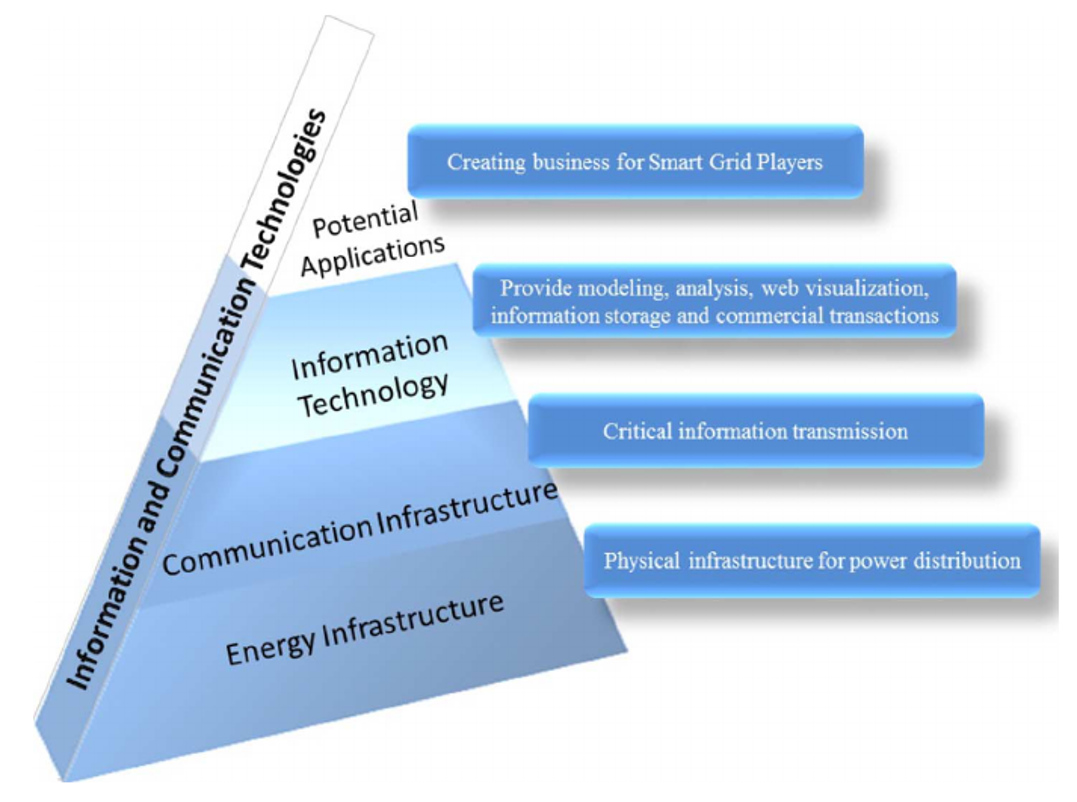
\includegraphics[scale=0.3, natwidth=1003,natheight=490]{imgs/ict.png}}
\caption{Smart Grid framework}\label{fig:1}
\end{figure}

% http://ieeexplore.ieee.org/stamp/stamp.jsp?tp=&arnumber=6298960 